\documentclass{mythesis}

\usetikzlibrary{patterns}

\usepackage{titling}

\title{Inpainting mit Eulers Elastica}
\author{Stephan Hilb}


%\DeclareDocumentCommand{\thesection}{}{\arabic{section}}
%\DeclareDocumentCommand{\thesubsection}{}{\thesection.\arabic{subsection}}

% "such that"
\DeclareDocumentCommand{\st}{}{\mathbin{|}}

\DeclareDocumentCommand{\Edat}{}{E_{\mathrm{dat}}}
\DeclareDocumentCommand{\Eimg}{}{E_{\mathrm{img}}}

\DeclareDocumentCommand{\BV}{}{\mathord{\mathrm{BV}}}


\tikzset{missing/.style={dashed,pattern=checkerboard,pattern color=red!15}}

\colorlet{fg}{black}
\colorlet{bg}{white}


\begin{document}

%\usepackage{titling}

\begin{titlepage}
  \begin{center}
    ~\par\vspace{4em}
    {
      \fontsize { 16pt } { 16pt } \selectfont
      Masterarbeit
    }
    \par\vspace{3em}
    {
      \fontsize { 24pt } { 24pt } \selectfont \sffamily \bfseries
      \thetitle
    }
    \par\vspace{3em}
    {
      \fontsize { 16pt } { 16pt } \selectfont \scshape
      \theauthor
    }
    \par\vspace{1.5em}
    {
      \fontsize { 14pt } { 14pt } \selectfont %\scshape
      \today
    }
    \par\vspace{4.5em}
    {
    }
    \par\vspace{8em}
    {
      \fontsize { 14pt } { 14pt } \selectfont \scshape
      Universität Stuttgart
    }
    \par\vspace{1em}
    {
      \fontsize { 14pt } { 14pt } \selectfont %\scshape
      Institut für Angewandte Analysis und Numerische Simulation
    }
    \par\vspace{1em}
    {
      \fontsize { 14pt } { 14pt } \selectfont %\scshape
      Betreuer:
      Dr. Claus J. Heine,
      Dr. Andreas Langer
    }
  \end{center}
\end{titlepage}

\chapter*{Zusammenfassung}

Die Zielsetzung, fehlende Teile eines Bildes zu rekonstruieren – auch „Inpainting“ genannt – lässt sich als Minimierung eines
Funktionals für das Gesamtbild modellieren, bestimmt durch ein Datenmodell, das die Übereinstimmung mit dem ursprünglichen Bild auf dem bekannten Gebiet kontrolliert, und einem Bildmodell, welches maßgebend für die Güte der Rekonstruktion ist.

Das Euler Elastica Bildmodell, welches die Niveaulinien eines Bildes nach dem Vorbild elastischer Stäbe modelliert, bietet ein vielversprechendes Bildmodell und kommt in dieser Arbeit zum Einsatz.
Für die numerische Minimierung wird eine bekannte “alternating direction“ Augmented Lagrange Methode angewandt und die entstehenden Teilprobleme erstmalig im Kontext der Finiten Elemente gelöst.


{
  \let\clearpage\relax
  \tableofcontents
  %\addtocentrydefault{chapter}{}{Inhaltsverzeichnis}
}
%\tableofcontents



\chapter{Einführung}

%
%\begin{itemize}
%    \item
%	Lösungsansätze für das EE inpainting model in der Literatur
%\end{itemize}
%
%Mit Blick auf \ref{fig:setting} führen wir zunächst Begrifflichkeiten ein.

\begin{definition} \label{def:image}
    Ein \emphdef{Bild} ist eine Abbildung $u: \Omega \to F$, wobei $\Omega \subset \R^d$
    \emphdef{Trägermenge} genannt wird und $F$ \emphdef{Farbraum}.
    Für einen festen Farbraum $F$ sei $I_X$ die Menge der Bilder mit Trägermenge $X$.
    \begin{note}
	Wir betrachten im weiteren Verlauf Graustufenbilder und setzen daher stets $F := [0,1]$ (mit der
	Interpretation: $0$ entspricht „schwarz“ und $1$ „weiß“).
    \end{note}
\end{definition}

Wann immer man Strukturen oder geometrische Eigenschaften in solchen Bildern untersuchen möchte, ist man dazu geneigt diese Definition einzuschränken (indem man z.B. eine Form von Differenzierbarkeit fordert).
Obwohl dies oft im Widerspruch zu den üblichen Eigenschaften von Bildern steht (z.B. Unstetigkeiten an Kanten und Konturen), werden wir dies später an den entsprechenden Stellen tun.

\begin{figure}[ht]
    \centering
    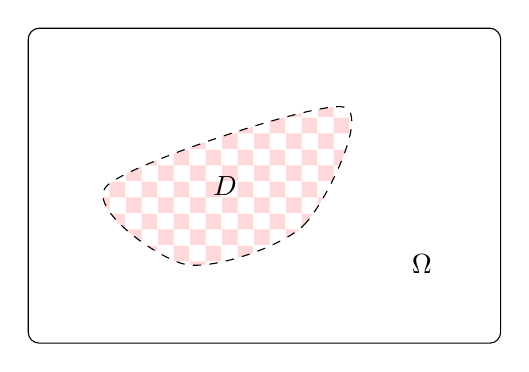
\begin{tikzpicture}
	\draw[rounded corners] (0,0) rectangle (6,4);
	\draw (5,1) node {$\Omega$};
	\draw[missing] plot[smooth cycle] coordinates {(2,1) (3.5,1.5) (4,3) (1,2)};
	\draw (2.5,2) node {$D$};
    \end{tikzpicture}
    \caption{Typische Inpainting-Situation}
    \label{fig:inpainting_setting}
\end{figure}

Beim Inpainten gehen wir von einem gegebenen Bild $u^0: \Omega \setminus D \to [0,1]$ und einem \emphdef{Inpainting-Bereich}
$D \subset \Omega$ aus (siehe \ref{fig:inpainting_setting}. Ziel ist nun eine Rekonstruktion $u: \Omega \to [0,1]$, die optisch „möglichst gut zu $u^0$ passt“.

Wir werden „möglichst gut“ durch die Minimierung eines Energiefunktionals $E[u]$ bestehend aus einem Datenmodell (engl. “data model”) und einem Bildmodell (engl. “image prior model”) ersetzen.
Der Bayes'sche Ansatz liefert hierfür eine schmackhafte Motivation.


\section{Das Bayes'sche Prinzip}

Es seien hier $I_\Omega$, $I_{\Omega \setminus D}$ endlich.
Dies ist beispielsweise der Fall, wenn $\Omega \subset \Z^d$ beschränkt und $F$ endlich ist, was bei praktisch allen digitalen Bildern zwingend ist.

\begin{samepage}
Geht man davon aus, dass $u^0$ zu einem ursprünglichen, vollständigen Bild $u$ gehört, so lässt sich die Entstehung von $u^0$ als Zufallsexperiment in zwei Schritten modellieren:
\begin{enumerate}
    \item
	Auftreten von $u$ als Bild im (diskreten) Wahrscheinlichkeitsraum $(I_\Omega, 2^{I_\Omega}, P_{\mathrm{img}})$, \nopagebreak
    \item
        Zustandekommen von $u^0$ als Beobachtung von $u|_{\Omega \setminus D}$ in $(I_{\Omega \setminus D}, 2^{I_{\Omega \setminus D}}, P_{\mathrm{dat},u})$.
\end{enumerate}
\end{samepage}
Wir betrachten dazu den diskreten Wahrscheinlichkeitsraum $\scr P := (I_\Omega \times I_{\Omega\setminus D}, 2^{I_\Omega \times I_{\Omega\setminus D}}, P)$ mit der sogenannten A-Posteriori-Wahrscheinlichkeitsverteilung
\begin{math}
    P(u, u^0) := P_{\mathrm{img}}(u) \cdot P_{\mathrm{dat},u^0}(u)
\end{math}
In diesem Raum besitzt $P_{\mathrm{dat},u^0}(u)$ die gewünschte Interpretation als bedingte Wahrscheinlichkeit $P(u^0|u)$:
\begin{math}
    P(u) &= P_{\mathrm{img}}(u), \\
    P(u^0|u) &= \frac{P(u, u^0)}{P(u)} = P_{\mathrm{dat},u^0}(u),
\end{math}
wobei wir $u$ und $u^0$ mit $\Set{u} \times I_{\Omega \setminus D}$, bzw. $I_\Omega \times \Set{u_0}$ identifizieren.
Dieser Raum erlaubt uns die Berechnung der bedingten Wahrscheinlichkeit
\begin{math}
    P(u|u^0) &= \frac{P(u, u^0)}{P(u^0)}
    = \frac{P(u^0|u) \cdot P(u)}{P(u^0)}.
\end{math}
Dieser einfache Zusammenhang zwischen den bedingten Wahrscheinlichkeiten ist auch als \emph{Satz von Bayes} bekannt.

Beim Inpainten ist $P(u^0)$ ist konstant und $P(u|u^0)$ die Wahrscheinlichkeit, dass $u$ die korrekte Rekonstruktion von $u^0$ ist, also maximieren wir
\begin{math}
    P(u|u^0) = \const \cdot P_{\mathrm{dat},u^0}(u) \cdot P_{\mathrm{img}}(u).
\end{math}
Wir können nun auf beiden Seiten $-\log(\argdot)$ anwenden und ein äquivalentes, aber durchaus handlicheres Problem in Energie-Form betrachten.

Für gegebenes $u^0$, $D$ minimieren wir also die Summe aus Datenterm und Bildterm (die additive Konstante ist für das Minimieren irrelevant)
\begin{math}
    E[u] = \Edat[u] + \Eimg[u].
\end{math}
Die Wahlen von $\Edat[u]$ und $\Eimg[u]$, welche den Wahrscheinlichkeitsverteilungen in unserem zweistufigen Zufallsmodell entsprechen, sind durch das Datenmodell, bzw. das Bildmodell festgelegt.


\section{Das Datenmodell}

Naheliegend ist der Gedanke, als Datenmodell lediglich $u|_{\Omega \setminus D} = u^0|_{\Omega \setminus D}$ zu fordern.
Damit würden feste Randbedingungen für das Minimieren auf $D$ vorgegeben werden.
In der Praxis sind Bilder jedoch meist mit Rauschen, Unschärfe oder anderen Artefakten versetzt, sei es aufgrund technischer Aufnahmebedingungen, natürlichen Zerfalls, digitaler Kompressionsartefakte oder aus anderen Gründen.
Das Datenmodell erlaubt es zu definieren, auf welche Weise $u|_{\Omega \setminus D}$ beim Inpainten an das vorliegende Bild $u^0$ angepasst werden soll und ermöglicht es solche Verunreinigungen auszugleichen.

Wir nutzen den bekannten Datenterm aus \cite{rudin1992nonlinear}, welcher die quadrierte $L^2$-Norm verwendet:
\begin{math}
    \Edat[u] = \frac{\eta}{2} \int_{\Omega \setminus D} |u - u^0|^2,
\end{math}
wobei $\eta \in \R_{> 0}$ die spätere Gewichtung des Datenterms zum Bildterm kontrolliert.

Es ist bekannt \cite[§4.5]{chan2005image}, dass dieser Datenterm gut geeignet ist, wenn das Orginalbild mit Gaus'schem Rauschen versetzt ist, modelliert als $u^0 = u|_{\Omega \setminus D} + \eta$.
Für Schwarz/Weiß Rauschen (auch “salt-and-pepper noise” oder “impulse noise” gennant) ist die Wahl einer $L^1$-Norm zu bevorzugen, wie in \cite{nikolova2004variational} gezeigt.

Denkbar wären auch Datenmodelle wie $u^0 = K[u|_{\Omega\setminus D}] + \epsilon$ für einen Glättungsoperator $K$.
Solche Modelle würden es erlauben, Unschärfe zu reduzieren, siehe z.B. \cite{rudin1994total}.


\section{Das Bildmodell}

Da der Datenterm sich auf $\Omega \setminus D$ beschränkt hat, trägt das Bildmodell die Hauptrolle bei der eigentlichen Bildrekonstruktion innerhalb von $D$.
Man beachte, dass das Bildmodell unabhängig von $D$ ist (man erinnere sich an das Bayes-Prinzip) und auch für $D = \emptyset$ (z.B. Denoising) die Rekonstruktion des ursprünglichen Bildes verbessern kann.
In der Literatur zum Denoising wird $\Eimg[u]$ daher auch als “regularization term” bezeichnet.

\begin{figure}[ht]
    \begin{subfigure}[b]{0.33\textwidth}
	\centering
        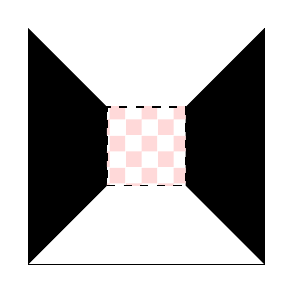
\begin{tikzpicture}
	    \draw[clip] (0,0) rectangle (3,3);
	    \fill[bg] (0,0) rectangle (3,3);
	    \fill[fg] (0,0) -- (1,1) -- (1,2) -- (0,3) -- cycle;
	    \fill[fg] (3,0) -- (3,3) -- (2,2) -- (2,1) -- cycle;
	    \draw[missing] (1,1) -- (2,1) -- (2,2) -- (1,2) -- cycle;
        \end{tikzpicture}
    \end{subfigure}%
    \begin{subfigure}[b]{0.33\textwidth}
	\centering
        
\begin{tikzpicture}
	    \draw[clip] (0,0) rectangle (3,3);
	    \fill[fg] (0,0) rectangle (3,3);
	    \fill[bg] (0,0) -- (3,0) -- (2,1) -- (1,1) -- cycle;
	    \fill[bg] (0,3) -- (1,2) -- (2,2) -- (3,3) -- cycle;
        \end{tikzpicture}
    \end{subfigure}%
    \begin{subfigure}[b]{0.33\textwidth}
	\centering
        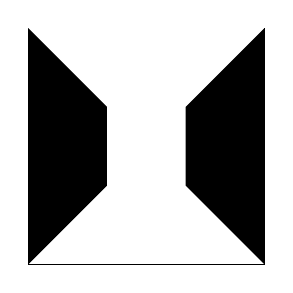
\begin{tikzpicture}
	    \draw[clip] (0,0) rectangle (3,3);
	    \fill[bg] (0,0) rectangle (3,3);
	    \fill[fg] (0,0) -- (1,1) -- (1,2) -- (0,3) -- cycle;
	    \fill[fg] (3,0) -- (3,3) -- (2,2) -- (2,1) -- cycle;
        \end{tikzpicture}
    \end{subfigure}
    \caption{Bewertungsschwierigkeiten: welches der beiden vollständigen Bildern ist wahrscheinlicher?}
    \label{fig:inpainting_non_unique}
\end{figure}

Zunächst macht man sich schnell anhand von einfachen Beispielen klar, dass die Wahl eines guten Bildmodells keineswegs einfach oder eindeutig ist, da die Bildbewertung oft von der menschlichen Interpretation abhängt.
Welche der beiden vollständigen Bilder aus Abbildung \ref{fig:inpainting_non_unique} ein Betrachter eher für richtig hält, hängt davon ab, ob er Hell oder Dunkel für vordergründiger hält.

\begin{figure}[ht]
    \begin{subfigure}[b]{0.33\textwidth}
	\centering
        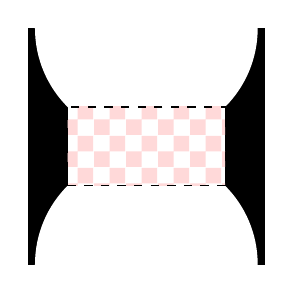
\begin{tikzpicture}
	    \draw[clip] (0,0) rectangle (3,3);
	    \fill[fg] (0,0) rectangle (3,3);
	    \fill[bg] (1.5,3) circle[radius=1.41421];
	    \fill[bg] (1.5,0) circle[radius=1.41421];
	    \fill[bg] (0.5,1) -- (2.5,1) -- (2.5,2) -- (0.5,2) -- cycle;
	    \draw[missing] (0.5,1) -- (2.5,1) -- (2.5,2) -- (0.5,2) -- cycle;
        \end{tikzpicture}
    \end{subfigure}%
    \begin{subfigure}[b]{0.33\textwidth}
	\centering
        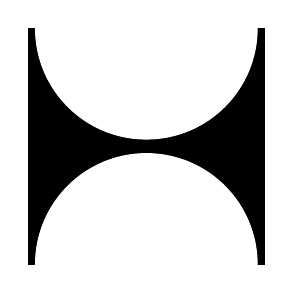
\begin{tikzpicture}
	    \draw[clip] (0,0) rectangle (3,3);
	    \fill[fg] (0,0) rectangle (3,3);
	    \fill[bg] (1.5,3) circle[radius=1.41421];
	    \fill[bg] (1.5,0) circle[radius=1.41421];
        \end{tikzpicture}
    \end{subfigure}%
    \begin{subfigure}[b]{0.33\textwidth}
	\centering
        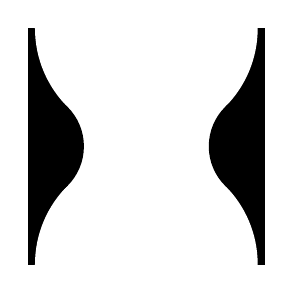
\begin{tikzpicture}
	    \draw[clip] (0,0) rectangle (3,3);
	    \fill[fg] (0,0) rectangle (3,3);
	    \fill[bg] (1.5,3) circle[radius=1.41421];
	    \fill[bg] (1.5,0) circle[radius=1.41421];
	    \fill[bg] (0.5,1) -- (2.5,1) -- (2.5,2) -- (0.5,2) -- cycle;
	    \fill[fg] (0,1.5) circle[radius=0.70710];
	    \fill[fg] (3,1.5) circle[radius=0.70710];
        \end{tikzpicture}
    \end{subfigure}
    \caption{Kurze Niveaulinien (rechts) werden bevorzugt}
    \label{fig:inpainting_prefer_short}
\end{figure}

%\begin{figure}[ht]
%    \begin{subfigure}[b]{0.33\textwidth}
%	\centering
%        \begin{tikzpicture}
%	    \draw[clip] (0,0) rectangle (3,3);
%	    \fill[fg] (0,0) rectangle (3,3);
%	    \fill[bg] (1.5,3) circle[radius=1.11803];
%	    \fill[bg] (1.5,0) circle[radius=1.11803];
%	    \fill[bg] (1,1) -- (2,1) -- (2,2) -- (1,2) -- cycle;
%	    \draw[missing] (1,1) -- (2,1) -- (2,2) -- (1,2) -- cycle;
%        \end{tikzpicture}
%    \end{subfigure}%
%    \begin{subfigure}[b]{0.33\textwidth}
%	\centering
%        \begin{tikzpicture}
%	    \draw[clip] (0,0) rectangle (3,3);
%	    \fill[fg] (0,0) rectangle (3,3);
%	    \fill[bg] (1.5,3) circle[radius=1.11803];
%	    \fill[bg] (1.5,0) circle[radius=1.11803];
%        \end{tikzpicture}
%    \end{subfigure}%
%    \begin{subfigure}[b]{0.33\textwidth}
%	\centering
%        \begin{tikzpicture}
%	    \draw[clip] (0,0) rectangle (3,3);
%	    \fill[fg] (0,0) rectangle (3,3);
%	    \fill[bg] (1.5,3) circle[radius=1.11803];
%	    \fill[bg] (1.5,0) circle[radius=1.11803];
%	    \fill[bg] (1,1) -- (2,1) -- (2,2) -- (1,2) -- cycle;
%	    \fill[fg] (0.75,1.5) circle[radius=0.55902];
%	    \fill[fg] (2.25,1.5) circle[radius=0.55902];
%        \end{tikzpicture}
%    \end{subfigure}
%    \caption{Krümmungsarme Niveaulinien (mitte) werden bevorzugt}
%    \label{fig:inpainting_prefer_non_curved}
%\end{figure}

\begin{figure}[ht]
    \begin{subfigure}[b]{0.33\textwidth}
	\centering
        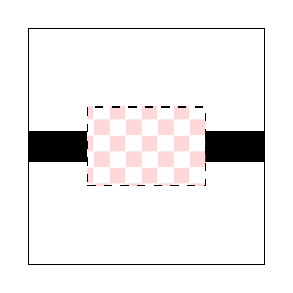
\begin{tikzpicture}
	    \draw[clip] (0,0) rectangle (3,3);
	    \fill[fg] (0,1.3) rectangle (3,1.7);
	    \fill[bg] (0.75,1) -- (2.25,1) -- (2.25,2) -- (0.75,2) -- cycle;
	    \draw[missing] (0.75,1) -- (2.25,1) -- (2.25,2) -- (0.75,2) -- cycle;
        \end{tikzpicture}
    \end{subfigure}%
    \begin{subfigure}[b]{0.33\textwidth}
	\centering
        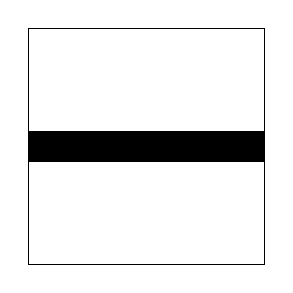
\begin{tikzpicture}
	    \draw[clip] (0,0) rectangle (3,3);
	    \fill[fg] (0,1.3) rectangle (3,1.7);
        \end{tikzpicture}
    \end{subfigure}%
    \begin{subfigure}[b]{0.33\textwidth}
	\centering
        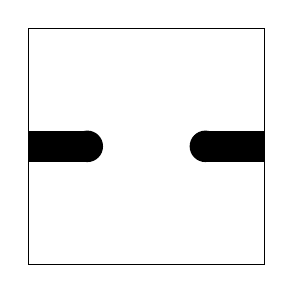
\begin{tikzpicture}
	    \draw[clip] (0,0) rectangle (3,3);
	    \fill[fg] (0,1.3) rectangle (3,1.7);
	    \fill[bg] (0.75,1) -- (2.25,1) -- (2.25,2) -- (0.75,2) -- cycle;
	    \fill[fg] (0.75,1.5) circle[radius=0.2];
	    \fill[fg] (2.25,1.5) circle[radius=0.2];
        \end{tikzpicture}
    \end{subfigure}
    \caption{Krümmungsarme Niveaulinien (mitte) werden bevorzugt}
    \label{fig:inpainting_prefer_non_curved}
\end{figure}

Wir betrachten nun zweidimensionale Bilder $d = 2$.
Anhand von Abbildungen \ref{fig:inpainting_prefer_non_curved} und \ref{fig:inpainting_prefer_non_curved} sieht man, dass in der Regel Bilder bevorzugt werden, bei denen die Kanten (oder Niveaulinien) des Bildes möglichst kurz und gering gekrümmt sind.
Die Niveaulinien eines Bildes stellen auf diese Weise in vielen Fällen eine brauchbare Bewertungsgrundlage dar.
Legt man eine geeignete Bewertung für die Niveaulinien eines Bildes (im Sinne eines Energiefunktionals) fest, so liefert die Summation über alle Höhenlinien eine Bewertung des Gesamtbildes.
Diese Methode wird \emphdef{Levelset-Methode} genannt (siehe Kapitel \ref{chap:image_model}).

Das Bildmodell in dieser Arbeit nutzt die Levelset-Methode und wählt für jede Niveaulinie $\gamma$ die \emphdef{Elastica Energie}
\begin{math}
    \int_{\gamma} \alpha + \beta \kappa^2 \di[s].
\end{math}
Eine Kurve, die diese Energie (unter geeigneten Randbedingungen) minimiert, wird \emphdef{Elastica} genannt.
In der Physik hat sie die Interpretation der Biegeenergie eines elastischen Stabes.
Umfangreiche Herleitungen finden sich in \cite{love1920treatise} und \cite{antman2005problems}, während obige Form der Elastica Energie aus \cite{birkhoff1965nonlinear} stammt.

Die Levelset-Methode liefert uns schließlich für unser Bildmodell (näheres in Kapitel \ref{chap:image_model})
\begin{math}
    \Eimg[u] = \int_{\Omega} \Big(\alpha + \beta (\nabla \cdot \frac{\nabla u}{\nabla u})^2\Big)|\nabla u| \di[x].
\end{math}
Es sei bemerkt, dass dieses geometrische Inpaintingmodell nicht darauf ausgelegt ist wiederkehrende Strukturen zu reproduzieren, die deutlich kleiner als der Inpaintingbereich $D$ sind (siehe Abbildung \ref{fig:inpainting_texture}).
%Wiederkehrende Strukturen außerhalb $D$ werden nicht innerhalb $D$ fortgesetzt.
Hierfür gibt es sogenanntes “texture based inpainting” mit zahlreichen stochastischen Methoden (siehe z.B. \cite{criminisi2004region}).

\begin{figure}[ht]
    \begin{subfigure}[b]{0.33\textwidth}
	\centering
        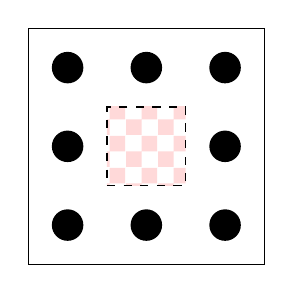
\begin{tikzpicture}
	    \draw[clip] (0,0) rectangle (3,3);
	    \foreach \x in {0.5, 1.5, 2.5}
		\foreach \y in {0.5, 1.5, 2.5}
		    \fill (\x,\y) circle[radius=0.2];
	    \fill[bg] (1,1) -- (2,1) -- (2,2) -- (1,2) -- cycle;
	    \draw[missing] (1,1) -- (2,1) -- (2,2) -- (1,2) -- cycle;
        \end{tikzpicture}
    \end{subfigure}%
    \begin{subfigure}[b]{0.33\textwidth}
	\centering
        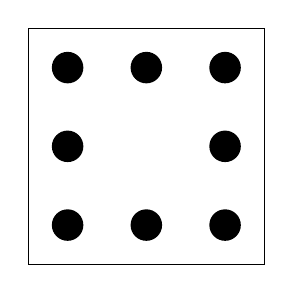
\begin{tikzpicture}
	    \draw[clip] (0,0) rectangle (3,3);
	    \foreach \x in {0.5, 1.5, 2.5}
		\foreach \y in {0.5, 1.5, 2.5}
		    \fill (\x,\y) circle[radius=0.2];
	    \fill[bg] (1,1) -- (2,1) -- (2,2) -- (1,2) -- cycle;
        \end{tikzpicture}
    \end{subfigure}%
    \begin{subfigure}[b]{0.33\textwidth}
	\centering
        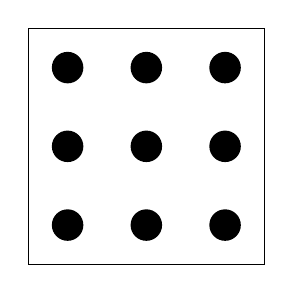
\begin{tikzpicture}
	    \draw[clip] (0,0) rectangle (3,3);
	    \foreach \x in {0.5, 1.5, 2.5}
		\foreach \y in {0.5, 1.5, 2.5}
		    \fill (\x,\y) circle[radius=0.2];
        \end{tikzpicture}
    \end{subfigure}
    \caption{Unser Bildmodell würde das mittlere Bild dem rechten vorziehen}
    \label{fig:inpainting_texture}
\end{figure}


\chapter{Das Euler Elastica Bildmodell} \label{chap:image_model}


Wir bereits in der Einführung angesprochen, wollen wir in diesem Kapitel die Elastica Kurve als Kurvenmodell für die Niveaulinien eines Bildes ansetzen, um daraus anschließend ein Bildmodell zu gewinnen.

\section{Die Euler Elastica}

In der Physik bezeichnet man einen festen Gegenstand in der Regel als elastisch, wenn es sich unter äußerer Krafteinwirkung deformiert und nach dem Entfernen dieser Kraft wieder in seine Ausgangsform zurückkehrt.
Die Frage, wie genau sich ein elastischer Gegenstand unter äußerer Krafteinwirkung verformt, ist im Allgemeinen stark materialabhängig und schwierig zu beantworten.

Die Wissenschaft hat mit der Zeit eine Reihe von Modellen entwickelt, um das Verhalten elastischer Gegenstände zu beschreiben.
Man erinnere sich beispielsweise an das Hookesche Gesetz aus der Schulphysik, welches zwischen Elongation eines Objektes (z.B. eine Spannfeder) in eine Richtung und der darauf einwirkenden Kraft einen linearen Zusammenhang herstellt.
Dieses Modell war jedoch eindimensional und reichte auch nicht aus, um größere Verformungen zu beschreiben, die sich nicht dem linearen Gesetz unterwerfen.

Euler hat schließlich (nach Vorarbeit von Bernoulli und anderen, siehe \cite{levien2008elastica}) 1744 in seinem Buch über variationelle Methoden \cite{euler1774methodus} ein Modell für planare elastische Stäbe fester Länge präsentiert.
Eine Elastica war demnach (in aktueller Notation) eine zweifach stetig differenzierbare, reguläre Kurve $\gamma: [0,L] \to \R^2$ fester Länge $L > 0$, festen Endpunkten $\gamma(0), \gamma(L)$ und festen Tangentenrichtungen $\dot \gamma(0), \dot \gamma(L)$, welche die totale quadrierte Krümmung
\begin{math}
    \int_\gamma \kappa^2 \di[s]
\end{math}
minimiert.
In seinem Werk löst Euler dieses Variationsproblem indem er alle zugehörigen kritischen Punkte (Kurven) klassifiziert und weiß darauf hin, dass das Modell bekannte Eigenschaften elastischer Stäbe reproduziert.

Neben ihrer geschmeidigen Form erbt die Elastica durch diese Formulierung auch viele schöne geometrische Eigenschaften der Krümmung, wie z.B. Invarianz unter euklidischen Transformationen.
In neuerer Zeit wurde die Elastica deshalb in der Numerik z.B. als Vorbild für Spline-Interpolationen oder wie in dieser Arbeit als Kurvenmodell für Levelsetmethoden in Betracht gezogen.
Man möchte sich dabei meist von der unhandlichen Randbedingung der festen Länge befreien und wählt folgende Definition.

\begin{definition}[Euler Elastica] \label{definition:elastica}
    Eine Kurve $\gamma \in C^2([0,1], \R^2)$ mit festen Endpunkten $\gamma(0) = p_0$, $\gamma(1) = p_1$ und Tangentenrichtungen $\dot\gamma(0) = t_0$, $\dot\gamma(1) = t_1$ heißt \emphdef{Elastica}, falls sie unter eben solchen zulässigen Kurven ein kritischer Punkt des Energiefunktionals
    \begin{math}
	\int_\gamma \alpha + \beta \kappa^2 \di[s]
    \end{math}
    ist.
    Diese Energie nennen wir auch \emphdef{Elastica Energie der Kurve $\gamma$}.
\end{definition}

Eine interessante Charakterisierung der Elastica liefert der folgende Satz.

\begin{proposition} \label{proposition:elastica_el}
    Eine Kurve $\gamma \in C^4([0,L], \R^2)$ mit Randbedingungen wie in Definition \ref{definition:elastica} ist eine Elastica genau dann, wenn die zugehörige Euler-Lagrange-Gleichung
    \begin{math}
	\beta\big(2\ddot\kappa + \kappa^3\big) - \alpha\kappa = 0
    \end{math}
    erfüllt ist.
    \begin{proof}
	Sei $\gamma$ stets in Bogenlänge parametrisiert mit Tangente $e_1$ und Normale $e_2$.
        Die Kurvenenergie sei gegeben durch $F[\gamma] := \int_\gamma \alpha + \beta \kappa^2 \di[s]$.
	Wir bedienen uns der Variationsrechnung und lösen
	\begin{math}
	    \ddx[\epsilon]|_{\epsilon=0} F[\gamma + \epsilon \phi e_2] = 0,
	\end{math}
	wobei $\phi \in C^2([0,L], \R^2)$ eine Variation in Normalenrichtung $e_2$ darstellt.
	Sei $\gamma_\epsilon = \gamma + \epsilon \phi e_2$.
	Die Krümmung $\kappa_\epsilon$ von $\gamma_\epsilon$ lässt sich parametrisierungsunabhängig durch $\kappa_\epsilon = \frac{\det(\dot\gamma_\epsilon, \ddot\gamma_\epsilon)}{|\dot\gamma_\epsilon|^3}$ darstellen.
	Wir berechnen nun
	\begin{math}
	    \dot \gamma_\epsilon &= t + \epsilon \dot \phi e_2 - \epsilon \phi \kappa e_1 \\
	    &= (1-\epsilon \phi \kappa)e_1 + \epsilon \dot \phi n, \\
	    \ddot \gamma_\epsilon &= (-\epsilon \dot \phi \kappa - \epsilon \phi \dot \kappa) e_1 + (1-\epsilon \phi \kappa) \kappa e_2 + \epsilon \ddot \phi n - \epsilon \dot \phi \kappa e_1 \\
	    &= (-2\epsilon \dot\phi \kappa - \epsilon \phi \dot \kappa) e_1 + (\epsilon \ddot \phi - \epsilon \phi \kappa^2 + \kappa) e_2, \\
	    \det(\dot\gamma_\epsilon, \ddot \gamma_\epsilon)
	    &=(1-\epsilon\phi\kappa)(\epsilon\ddot\phi - \epsilon\phi\kappa^2 + \kappa) + \epsilon \dot\phi(2 \epsilon \dot\phi \kappa - \epsilon\phi\dot\kappa),
	\end{math}
	und somit
	\begin{math}
	    \ddx[\epsilon]|_{\epsilon=0} |\dot\gamma_\epsilon|
	    &= \frac{1}{|\dot\gamma_0|} (\dot\gamma_0 \cdot \ddx[\epsilon] \dot\gamma_\epsilon) \\
	    &= e_1 \cdot (-\phi \kappa e_1 + \dot \phi e_2) \\
	    &= - \phi \kappa, \\
	    \ddx[\epsilon]|_{\epsilon=0} \det(\dot\gamma_\epsilon, \ddot\gamma_\epsilon)
	    &= -\phi \kappa^2 + (\ddot \phi - \phi\kappa^2) + \dot\phi \cdot 0 + 0 \cdot (2\dot\phi\kappa - \phi \dot\kappa) \\
	    &= \ddot\phi - 2\phi\kappa^2.
	\end{math}
	Zusammen ergibt sich
	\begin{math}
	    0 &= \ddx[\epsilon]|_{\epsilon = 0} F[\gamma_\epsilon] \\
	    &= \ddx[\epsilon]|_{\epsilon=0} \int_0^L (\alpha + \beta \kappa^2)|\dot\gamma_\epsilon| \di[\tau] \\
	    &= \int_0^L \alpha \ddx[\epsilon]|_{\epsilon = 0}|\dot\gamma_\epsilon| + \beta \ddx[\epsilon]|_{\epsilon = 0} \dfrac{\det(\dot\gamma_\epsilon, \ddot\gamma_\epsilon)^2}{|\dot\gamma_\epsilon|^5} \di[\tau] \\
	    &= \int_0^L -\alpha \kappa \phi + \beta \Big(2\kappa \ddx[\epsilon]|_{\epsilon=0} \det(\dot\gamma_\epsilon, \ddot\gamma_\epsilon) + 5\kappa^3 \phi \Big) \\
	    &= \int_0^L 2\beta\kappa \ddot\phi + \beta \kappa^3 \phi - \alpha\kappa\phi.
	\end{math}
	Partielle Integration unter Beachtung der Randbedingungen $\phi(0), \phi(1), \dot\phi(0), \dot\phi(L) = 0$ und Variationsrechnung führt schließlich auf
	\begin{math}
	    \beta(2\ddot\kappa + \kappa^3) - \alpha \kappa = 0.
	\end{math}
    \end{proof}
\end{proposition}

TODO: kinetische Betrachtung


\section{Die Levelset-Methode}

Die Idee der Levelset-Methode in der Numerik ist es, Berechnungen auf Kurven (oder Flächen) mit Hilfe einer sogenannten Levelset-Funktion in kartesischen Koordinaten durchführen zu können, ohne jeweils eine konkrete Parametrisierung der Kurven zu benötigen.
Die Levelset-Funktion enthält dabei die zu betrachtenden Kurven als Niveaulinien.

\begin{definition}
    Sei $\Omega \subset \R^2$ offen, $\gamma \in C^1([0,1], \Omega)$ eine reguläre Kurve und $\lambda \in \R$.
    Eine stetig differenzierbare Abbildung $u: \Omega \to \R^2$ heißt \emphdef{$\lambda$-Levelset-Funktion} für $\gamma$, falls für alle $t \in [0,1]$ gilt
    \begin{enumerate}[i)]
        \item
	    $(u \circ \gamma)(t) = \lambda$ und
	\item
	    $\det(\dot \gamma(t), \nabla u(\gamma(t))) > 0$.
    \end{enumerate}
    Wir nennen $\gamma$ auch \emphdef{$\lambda$-Levelset-Kurve} zu $u$.
    \begin{note}
        Die zweite Bedingung $\det(\dot \gamma, \nabla u) > 0$ sichert uns eine einheitliche Orienterung der Kurve.
    \end{note}
\end{definition}

Viele von $\gamma$ abhängige Größen können nun auch durch $u$ dargestellt werden, wie z.B. die Einheitsnormale $e_2$ von $\gamma$ an einem Punkt $x = \gamma(t)$.
Einmaliges Ableiten von $(u \circ \gamma)(t) = 0$ nach $t$ liefert nämlich
\begin{math}
    0 = \nabla u(\gamma(t)) \cdot \dot \gamma(t).
\end{math}
Falls $\nabla u(x) \neq 0$, so muss also $\frac{\nabla u(x)}{|\nabla u(x)|} = e_2(t)$, wobei das Vorzeichen durch $\det(\dot\gamma, \nabla u) > 0$ sichergestellt ist.
Dies motiviert folgende Definition.

\begin{definition}
    Für eine Abbildung $u \in C^1(\Omega, [0,1])$ mit $\nabla u(x) \neq 0$ für alle $x \in \Omega$ sei
    \begin{math}
        n: \Omega &\to \R^2 \\
	x &\mapsto \frac{\nabla u(x)}{|\nabla u(x)|}
    \end{math}
    das \emphdef{Normalenfeld} von $u$.
\end{definition}

Die Elastica Energie $\int_\gamma \alpha + \beta \kappa^2 \di[s]$ im Hinterkopf wollen wir nun die Krümmung $\kappa$ der Niveaulinie eines Bildes durch $u$ darstellen.

\begin{lemma}
    Sei $\Omega \subset \R^2$, $\gamma \in C^2([0,1], \Omega)$ regulär und $u \in C^2(\Omega, [0,1])$ eine zugehörige Levelset-Funktion mit Normalenfeld $n: \Omega \to \R^2$ und $\nabla u \neq 0$ auf $\Omega$.
    Dann gilt für alle $t \in [0,1]$, $x := \gamma(t)$
    \begin{math}
	\kappa(t) = - \nabla \cdot n(x) = - \nabla \cdot \frac{\nabla u(x)}{|\nabla u(x)|}.
    \end{math}
    \begin{note}
	Allgemeiner beschreibt $-\nabla \cdot n$ in der Differentialgeometrie die mittlere Krümmung einer Fläche mit Normale $n$.
    \end{note}
    \begin{proof}
        Seien $e_1, e_2$ die Einheitstangente und Einheitsnormale von $\gamma$,
       	dann gilt für die Krümmung $\kappa$ nach den Frenet-Serret Formeln
	\begin{math}
	    \Vector*{\dot e_1 & \dot e_2} = \Matrix*{0 & \kappa \\ -\kappa & 0} \Vector*{e_1 & e_2}.
	\end{math}
	Wegen $e_2 = n \circ \gamma$ erhalten wir gemäß Kettenregel
	\begin{math}
	    \kappa = - \dot e_2 \cdot e_1 = -n' t \cdot t.
	\end{math}
	Außerdem zeigt sich durch Differenzieren von $n_1^2 + n_2^2 = 1$
	\begin{math}
	    n_1 \partial_1 n_1 + n_2 \partial_1 n_2 &= 0, \\
	    n_1 \partial_2 n_1 + n_2 \partial_2 n_2 &= 0.
	\end{math}
	Zusammen ergibt sich
	\begin{math}
	    -\kappa &= n' t \cdot t \\
	    &= \Matrix*{\partial_1 n_1 & \partial_2 n_1 \\ \partial_1 n_2 & \partial_2 n_2}
	       \Vector*{n_2 & -n_1} \cdot \Vector*{n_2 & -n_1} \\
	    &= n_2 (n_2 \partial_1 n_1 - n_1 \partial_2 n_1) - n_1 (n_2 \partial_1 n_2 - n_1 \partial_2 n_2) \\
	    &= n_2 (n_2 \partial_1 n_1 + n_2 \partial_2 n_2) + n_1 (n_1 \partial_1 n_1 + n_1 \partial_2 n_2) \\
	    &= (n_1^2 + n_2^2) (\partial_1 n_1 + \partial_2 n_2) \\
	    &= \nabla \cdot n,
	\end{math}
	also $\kappa = - \nabla \cdot n$.
    \end{proof}
\end{lemma}

Wir haben damit folgende Darstellung für die Elastica Energie einer Kurve $\gamma$ mit Levelset-Funktion $u$:
\begin{math}
    \int_\gamma \alpha + \beta (\nabla \cdot \frac{\nabla u}{|\nabla u|})^2 \di[s].
\end{math}
Um nun ein Funktional für das Gesamtbild zu erhalten, werden wir über alle Levelset-Kurven summieren.
Das Werkzeug dafür ist die sogenannte Coarea-Formel, welche wir hier in zurechtgeschnittener Variante präsentieren.

\begin{proposition}[Coarea-Formel für glatte Bilder] \label{satz:coarea}
    Sei $f \in L^1(\Omega, \R)$ und seien $\gamma_\lambda \in C^1([0,1], \Omega)$ $\lambda$-Levelset-Kurven zu einem Bild $u \in C^1(\Omega, [0,1])$, sodass $\im \gamma_\lambda = \Set{x & u(x) = \lambda}$.
    Dann gilt
    \begin{math}
	\int_0^1 \int_{\gamma_\lambda} f \circ \gamma_\lambda \di[s] \di[\lambda]
	= \int_\Omega f |\nabla u| \di[x]
    \end{math}
    \begin{note}
        Durch entsprechende Zerlegung des Gebiets und wegen der Additivität der Integrale können wir hiermit auch Fälle abdecken, bei denen die Levelsets aus mehreren disjunkten Kurven bestehen.
    \end{note}
    \begin{proof}
        Für eine wesentlich allgemeinere Formulierung mit Beweis, siehe \cite[§3.4]{evans2015measure}.
    \end{proof}
\end{proposition}


\section{Das Euler Elastica Inpaintingmodell}


Die Coarea-Formel motiviert nun die folgende Definition der Euler Elastica Bildenergie.

\begin{definition}
    Für $u \in C^2(\Omega, [0,1])$ mit $\nabla u \neq 0$ auf $\Omega$ ist das Euler Elastica Bildmodell festgelegt durch die Minimierung der \emphdef{Elastica Bildenergie}
    \begin{math}
	\Eimg[u] = \int_\Omega \Big(\alpha + \beta (\nabla \cdot \frac{\nabla u}{|\nabla u|})^2\Big)|\nabla u| \di[x].
    \end{math}
    \begin{note}
	\begin{itemize}
	    \item
		In der Regel ignoriert man die Forderung nach $\nabla u \neq 0$ und nutzt die Konvention, dass in diesem Fall der Integrand gleich null ist.
	    \item
		Obige Formulierung ließe sich prinzipiell auch für $\Omega \subset \R^d$ mit $d > 2$ lesen.
		Anmerkungen dazu finden sich in \cite{ambrosio2003direct}.
	    \item
		Man kann diese Energie durch geeignete Methoden auch auf $L^1(\Omega, [0,1])$ erweitern, wie in \cite{ambrosio2003direct}:
		\begin{math}
		    \_E(u) := \inf \Set{ \liminf_{C^2 \ni u_h \to u} E(u_h) }.
		\end{math}
	\end{itemize}
    \end{note}
\end{definition}

\begin{remark}[TV-Bildmodell]
    Aus dem Elastica Bildmodell erhält man für $\alpha = 1, \beta = 0$ das bekannte TV-Bildmodell, welches für ein Bild $u \in C^2(\Omega, [0,1])$ die \emphdef{totale Variation}
    \begin{math}
	V_\Omega(u) := \int_\Omega |\nabla u| \di[x]
    \end{math}
    minimiert.
    Mit Blick auf die Coarea-Formel entsteht dieses Bildmodell aus einem Kurvenmodel, welches die Energie $\int_\gamma \di[s] = L(\gamma)$ minimiert.
    Das TV-Modell wird oft zum Entrauschen von Bildern verwendet, vor allem in der Signalverarbeitung für $d = 1$.

    In der Regel wird die Energie im allgemeineren Raum der Funktionen mit beschränkter totalar Variation
    \begin{math}
	\BV(\Omega) := \Set{u \in L^1(\Omega, [0,1]) & V_\Omega(u) < \infty}.
    \end{math}
    minimiert, wobei die totale Variation $V_\Omega(u)$ hier folgende Form hat (siehe \cite[§2.2]{chan2005image}):
    \begin{math}
	V_\Omega(u) := \sup\Set{ \int_\Omega u \nabla \cdot \phi & \phi \in C_0^1(\Omega,\R^d), \|\phi\|_{L^\infty(\Omega)} \le 1}.
    \end{math}
    Der Raum $\BV$ ist ein beliebter Funktionenraum in der Bildverarbeitung, da er allgemein genug ist, um fast alle konventionellen Bilder zu beschreiben und gleichzeitig die nötige geometrische Struktur bietet, um sinnvolle Bildmodelle zu definieren, näheres in \cite[§2.2]{chan2005image}.
\end{remark}

Erinnert man sich an das Bayes-Prinzip, so steht nun unser Inpaintingmodell fest.

\begin{definition} \label{definition:elastica_inpainting}
    Für gegebenes $u^0 \in L^2(\Omega, [0,1])$ und Inpaintingbereich $D \subset \Omega$ ist das \emphdef{Euler Elastica Inpaintingmodell} festgelegt durch die Minimierung der \emphdef{Elastica Inpaintingenergie}
    \begin{math}
        E[u]
	&= \Eimg[u] + \Edat[u] \\
	&= \int_\Omega \Big(\alpha + \beta (\nabla \cdot \frac{\nabla u}{|\nabla u|})^2\Big)|\nabla u| \di[x]
	  + \frac{\eta}{2} \int_{\Omega\setminus D} |u - u^0|^2 \di[x]
    \end{math}
    über $u \in C^2(\Omega, [0,1])$ für Konstanten $\alpha, \beta, \eta \in \R_{\ge 0}$.
    Der erste Integrand sei dabei Null, falls $\nabla u(x) = 0$.
\end{definition}


\chapter{Die “alternating direction” Methode}


\section{Motivation} % komplexität von euler-lagrange und numerische probl.


Für die numerische Implementierung des Elastica Inpaintingmodells aus Definition \ref{definition:elastica_inpainting} gibt es verschiedene Ansätze \cite{??}.

In diesem Kapitel nutzen wir Ideen und Notation aus \cite{??} und führen das unrestringierte Minimierungsproblem durch geignetes Einführen zusätzlicher Variablen und Nebenbedingungen auf ein restringiertes Minimierungsproblem.
Anschließend minimieren wir das zugehörige Augmented Lagrange Funktional (siehe Abschnitt \ref{section:augmented_lagrange}) mit Hilfe einer Alternating Direction Methode (siehe Abschnitt \ref{section:adm}).

\begin{lemma} \label{lemma:mp_constr}
    Seien $m, p \in \R^d$ zwei Vektoren mit $p \neq 0$.
    Dann sind die folgenden beiden Aussagen äquivalent:
    \begin{enumerate}[i)]
        \item
	    $|p| = m \cdot p$ und $|m| \le 1$,
	\item
	    $m = \frac{p}{|p|}$.
    \end{enumerate}
    \begin{proof}
        Aus ii) folgt trivialerweise i) durch Einsetzen von $m$.
	Es gelte also i) und setze $m = \frac{p}{|p|} + v$ für einen Vektor $v \in \R^d$.
	Dann rechnet man direkt
	\begin{math}
	    0 \le |v|^2 &= |m|^2 - 2 m \cdot \frac{p}{|p|} + 1
	    \le 1 - 2 + 1 = 0.
	\end{math}
	Somit muss $v = 0$ und $m = \frac{p}{|p|}$.
    \end{proof}
\end{lemma}

Mit Blick auf Lemma \ref{lemma:mp_constr} ist das Minimierungsproblem aus Definition \ref{definition:elastica_inpainting} äquivalent zu
\begin{math}[numbered] \label{eq:energy_splitted}
    \min_{\substack{u \in C^2(\Omega,[0,1]) \\ p,n,m \in C^1(\Omega, \R^d)}}
    &\scr E[u,p,m,n] = \int_\Omega \Big(\alpha + \beta(\nabla \cdot n)^2\Big)|p| + \frac{\eta}{2} \int_{\Omega \setminus D} |u - u_0|^2 \\
    &\quad \text{s.t.} \quad
	|p| = m \cdot p, \quad
	p = \nabla u, \quad
	n = m, \quad
	|m| \le 1.
\end{math}
%Hierbei sei $C^1_{|\argdot|\le 1}(\Omega, \R^d) := \Set{f \in C^1(\Omega, \R^d) & \forall x \in \Omega : |f(x)| \le 1}$.
Man beachte, dass wir mit der Formulierung \eqref{eq:energy_splitted} den Fall $\nabla u = 0$ nicht gesondert betrachten müssen.


\section{Augmented Lagrange}

TODO: Einführung + Formulierung




\begin{algorithm}[Augmented Lagrange] \label{alg:augmented_lagrange}
    \begin{samepage}
	\Input{$\scr E: X \to \R$, $e: X \to W$, $\lambda^0 = (\lambda^0_s)_{s=1}^S \in W$, $K \subset X$ konvex}\\
	\Output{Folge $(x^k)_{k\in\N}$ mit $\scr E[x^k] \to \min_x \scr E[x]$}
	\begin{algorithmic}
	    \For{$i = 0,1,\dotsc$}
		\State{$x^{i+1} \gets \argmin_{x \in K} \scr L[x, \lambda^i]$}
		\For{$s = 1,\dotsc,S$}
		    \State{$\lambda^{i+1}_s \gets \lambda^i_s + r_s e_s[x^{i+1}]$}
		\EndFor
	    \EndFor
	\end{algorithmic}
    \end{samepage}
    Hierbei sei
    \begin{math}
	\scr L[x, \lambda]
	:= \scr E[x] + \sum_{s=1}^S \Big( \lambda_s \cdot e_s[x_s] + r_s \|e_s[x_s]\|^2 \Big)
    \end{math}
\end{algorithm}


Für unser Problem aus \eqref{eq:energy_splitted} definieren wir das folgende Augmented Lagrange Funktional:
\begin{math}[numbered] \label{eq:energy_al}
    \scr L[u,p,m,n;\lambda_1, \lambda_2, \lambda_4]
    &= \int_\Omega \Big(\alpha + \beta (\nabla \cdot n)^2\Big)|p| + \frac{\eta}{2} \int_{\Omega\setminus D} |u - u^0|^2 \\
    &\quad + r_1 \int_\Omega (|p| - m\cdot p) + \int_\Omega \lambda_1 (|p| - m \cdot p) \\
    &\quad + \frac{r_2}{2} \int_\Omega |p - \nabla u|^2 + \int_\Omega \lambda_2 \cdot (p - \nabla u) \\
    &\quad + \frac{r_4}{2} \int_\Omega |n - m|^2 + \int_\Omega \lambda_4 \cdot (n - m).
\end{math}
Die Nebenbedingung $|m| \le 1$ fordern wir durch die Wahl von $K$ in Algorithmus \ref{alg:augmented_lagrange}.

Für den Penaltyterm zur Nebenbedingung $|p| = m \cdot p$ haben wir hier eine Änderung vorgenommen.
Wegen $m \in C^1_{|\argdot|\le 1}(\Omega, \R^d)$ ist $m \cdot p \le |m| |p| \le |p|$ und es handelt sich hier um $L^1$-Penalizing.
Die Modifikation wird es uns erlauben, einige der im nächsten Abschnitt aufkommenden Teilprobleme explizit zu lösen.



\section{Alternating Direction Method}

Statt das Augmented Lagrange Funktional in \eqref{eq:energy_al} nach $u, p, m, n$ gleichzeitig zu minimieren, minimieren wir es alternierend.

\begin{algorithm}[Alternating Direction Method] \label{alg:adm}
    \Input{$\scr L$, $x = (x_l)_{l=1}^L$, $\lambda$}\\
    \Output{Folge $(x^j)_{j \in \N}$ mit $\scr L[x^j, \lambda] \to \min_{x \in K} \scr L[x,\lambda]$}
    \begin{algorithmic}
	\For{$j = 1,\dotsc$}
	    \For{$t = 1,\dotsc, T$}
		\State{$x_t^{j+1} \gets \argmin_{x_t \in K_t} \scr L[x_1^{j+1}, \dotsc, x_t, \dotsc , x_T^j; \lambda]$}
	    \EndFor
	\EndFor
    \end{algorithmic}
\end{algorithm}

Die sich ergebenden Teilprobleme aus Algorithmus \ref{alg:adm} angewandt auf $\scr L$ aus \eqref{eq:energy_al} behandeln wir nun in den folgenden Abschnitten.

\subsection{Minimiere nach $u$}

Wir minimieren
\begin{math}
    \scr L[u] =
    \frac{\eta}{2} \int_{\Omega \setminus D} |u - u^0|^2
    + \frac{r_2}{2} \int_\Omega |p - \nabla u|^2
    + \int_\Omega \lambda_2 \cdot (p - \nabla u)
    + \const.
\end{math}
Variationsrechnung liefert als notwendige Bedingung
\begin{math}[numbered]
    0 &= \ddx[\epsilon] \scr L[u+\epsilon\phi] \\
    &= \eta \int_{\Omega\setminus D} (u - u^0) \phi + r_2 \int_\Omega (\nabla u - p) \cdot \nabla \phi - \int_\Omega \lambda_2 \cdot \nabla \phi \\
    &= \int_\Omega (r_2 \nabla u - r_2 p - \lambda_2) \cdot \nabla \phi + \eta \int_{\Omega\setminus D} (u - u^0)\phi.
\end{math}
Dies ist die schwache Form einer linearen PDE zweiter Ordnung, welche in Kapitel \ref{chap:numerics} numerisch gelöst wird.

\subsection{Minimiere nach $p$}

Wir minimieren nach geigneter quadratische Ergänzung und Vereinfachung
\begin{math}
    \scr L[p]
    &= \int_\Omega \Big(\alpha + \beta(\nabla \cdot n)^2\Big)|p|
	+ r_1 \int_\Omega (|p| - m \cdot p)
	+ \int_\Omega \lambda_1 (|p| - m \cdot p)
	+ \frac{r_2}{2} \int_\Omega |p - \nabla u|^2 \\
	&\qquad+ \int_\Omega \lambda_2 \cdot (p - \nabla u)
	+ \const\\
    &= \int_\Omega \underbrace{\Big(\alpha + \beta (\nabla \cdot n)^2 + r_1 + \lambda_1 \Big)}_{=:c}|p|
	+ \frac{r_2}{2} \int_\Omega \Big|p - \underbrace{(\nabla u + \frac{r_1 + \lambda_1}{r_2}m - \frac{\lambda_2}{r_2})}_{=:q}\Big|^2
	+ \const\\
    &= \int_\Omega c |p| + \frac{r_2}{2} \int |p -q|^2 + \const.
\end{math}

Mit dem folgenden Lemma \ref{lemma:soft_thresholding} erhalten wir also die explizite Lösung

\begin{math}[numbered]
    p &= \max\{0,1 - \frac{c}{r_2|q|}\} q
    \qquad \text{wobei} \qquad
    &\begin{aligned}
	c &= \alpha + \beta (\nabla \cdot n)^2 + r_1 + \lambda_1, \\
	q &= \nabla u + \frac{r_1 + \lambda_1}{r_2}m - \frac{\lambda_2}{r_2}.
    \end{aligned}
\end{math}

\begin{lemma}[Soft Thresholding] \label{lemma:soft_thresholding}
    Seien $p, q \in L^2(\Omega)$, $a, |p| \in L^1(\Omega)$ mit $a > 0$ fast überall.
    Dann wird das Funktional
    \begin{math}
        E[p] = \int_\Omega |p - q|^2 + \int_\Omega a |p|
    \end{math}
    minimiert durch
    \begin{math}
	\hat p = \max\Set{0, 1 - \frac{a}{2|q|}} q
    \end{math}
\end{lemma}

\subsection{Minimiere nach $m$}

Wir minimieren unter der Nebenbedingung $|m| \le 1$ nach geigneter quadratischer Ergänzung

\begin{math}
    \scr L[m]
    &= r_1 \int_\Omega (|p| - m \cdot p)
	+ \int_\Omega \lambda (|p| - m \cdot p)
	+ \frac{r_4}{2} \int_\Omega |n - m|^2
	+ \int_\Omega \lambda_4 \cdot (n - m)
	+ \const \\
    &= \frac{r_4}{2} \int_\Omega |w - m|^2 + \const,
\end{math}
wobei $w = \frac{(r_1 + \lambda_1)p + \lambda_4}{r_4} + n$.
Das folgende Lemma \ref{lemma:proj1} liefert nun die explizite Lösung
\begin{math}[numbered]
    m &:= \begin{cases}
	w & \text{für $|w| < 1$}, \\
	\frac{w}{|w|} & \text{für $|w| \ge 1$}.
    \end{cases}&
    \quad\text{wobei}\quad
    w &= \frac{(r_1 + \lambda_1)p + \lambda_4}{r_4} + n
\end{math}

\begin{lemma} \label{lemma:proj1}
    Seien $m, w \in L^2(\Omega)$.
    Dann wird das Funktional
    \begin{math}
        E[m] = \int_\Omega |w - m|^2
    \end{math}
    unter der Nebenbedingung $|m| \le 1$ minimiert durch
    \begin{math}
	\hat m := \begin{cases}
	    w & \text{für $|w| < 1$}, \\
	    \frac{w}{|w|} & \text{für $|w| \ge 1$}.
	\end{cases}
    \end{math}
\end{lemma}



\subsection{Minimiere nach $n$}

Wir minimieren
\begin{math}
    \scr L[n]
    &= \int_\Omega \Big(\alpha + \beta(\nabla \cdot \kappa)^2\Big)|p|
	+ \frac{r_4}{2} \int_\Omega |n - m|^2
	+ \int_\Omega \lambda_4 \cdot (n - m)
	+ \const.
\end{math}
Variationsrechnung liefert
\begin{math}[numbered]
    0 &= \ddx[\epsilon]|_{\epsilon = 0} \scr L[n + \epsilon \phi] \\
    &= \int_\Omega 2 \beta |p| (\nabla \cdot n)(\nabla \cdot \phi)
    + \int_\Omega (r_4 n - r_4 m + \lambda_4) \cdot \phi.
\end{math}
Dies ist die schwache Form einer linearen PDE zweiter Ordnung und wird ebenfalls in \ref{chap:numerics} gelöst.












%\begin{itemize}
%    \item
%	Operator-Splitting:
%	\begin{math}
%	    &\min_{v,u,m,p,n} \int_{\Omega} (\alpha + \beta(\nabla \cdot n)^2) |p| + \frac{\eta}{2} \int_{\Omega\setminus D} |v - u^0|^2 \\
%	    &\quad\mathrm{s.t.}\quad v = u, p = \nabla u, n = m, |p| = m \cdot p, |m| \le 1.
%	\end{math}
%    \item
%	Augmented Lagrange Funktional:
%	\begin{math}
%	    \scr L[v,u,m,p,n;\lambda_1,\lambda_2,\lambda_3,\lambda_4]
%	    &= \int_{\Omega} (\alpha + \beta(\nabla \cdot n)^2) |p| + \frac{\eta}{2} \int_{\Omega\setminus\Gamma} |v - u^0|^2 \\
%	    &\quad + r_1 \int_\Omega (|p| - m\cdot p) + \int_\Omega \lambda_1 (|p| - m \cdot p) \\
%	    &\quad + \frac{r_2}{2} \int_\Omega |p - \nabla u|^2 + \int_\Omega \lambda_2 \cdot (p - \nabla u) \\
%	    &\quad + \frac{r_3}{2} \int_\Omega (v - u)^2 + \int_\Omega \lambda_3 (v - u) \\
%	    &\quad + \frac{r_4}{2} \int_\Omega |n-m|^2 + \int_\Omega \lambda_4 \cdot (n - m) + \delta_{\ge 1}(m).
%	\end{math}
%    \item
%	Updates:
%	\begin{math}
%	    \lambda_1 &\gets \lambda_1 + r_1 (|p| - m\cdot p), \\
%	    \lambda_2 &\gets \lambda_2 + r_2 (p - \nabla u), \\
%	    \lambda_3 &\gets \lambda_3 + r_3 (v - u), \\
%	    \lambda_4 &\gets \lambda_4 + r_4 (n - m).
%	\end{math}
%\end{itemize}
%
%
%\begin{math}
%    \scr E_1[v]
%    &= \frac{\eta}{2} \int_{\Omega\setminus D} |v - u^0|^2 + \frac{r_3}{2} \int_\Omega (v-u)^2 + \int_\Omega \lambda_3(v - u)\\
%    \scr E_2[u]
%    &= \frac{r_2}{2} \int_\Omega |p - \nabla u|^2 + \int_\Omega \lambda_2 \cdot (p - \nabla u) + \frac{r_3}{2} \int_\Omega (v-u)^2 + \int_\Omega \lambda_3 (v-u) \\
%    \scr E_3[m]
%    &= r_1 \int_\Omega(|p| - m\cdot p) + \int_\Omega \lambda_1 (|p| - m \cdot p) + \frac{r_4}{2} \int_\Omega |n-m|^2 + \int_\Omega \lambda_4 \cdot (n-m) + \delta_{\ge 1}(m) \\
%    &= \frac{r_4}{2} \int_\Omega |x-m|^2 + \delta_{\ge 1}(m) + \const\\
%    \scr E_4[p]
%    &= \int_\Omega (\alpha + \beta(\nabla \cdot n)^2) |p| + r_1 \int_\Omega (|p| - m\cdot p) + \int_\Omega \lambda_1 (|p| - m\cdot p) \\
%    &\qquad + \frac{r_2}{2} \int_\Omega |p - \nabla u|^2 + \int_\Omega \lambda_2 \cdot (p - \nabla u) \\
%    &= \int_\Omega \Big(\alpha + \beta (\nabla \cdot n)^2 + r_1 + \lambda_1\Big) |p| + \frac{r_2}{2} \int_\Omega \Big| p - \big( \nabla u + \frac{r_1 + \lambda_1}{r_2} m - \frac{1}{r_2} \lambda_2 \big) \Big|^2 + \const\\
%    \scr E_5[n]
%    &= \int_\Omega (\alpha + \beta(\nabla \cdot n)^2 ) |p| + \frac{r_4}{2} \int_\Omega |n-m|^2 + \int_\Omega \lambda_4 \cdot (n - m)
%\end{math}
%
%\begin{enumerate}[1)]
%    \item
%	Minimiere
%	\begin{math}
%	    \scr E_1[v]
%	    = \frac{\eta}{2} \int_{\Omega\setminus D} |v - u^0|^2 + \frac{r_3}{2} \int_\Omega (v-u)^2 + \int_\Omega \lambda_3(v - u).
%	\end{math}
%	Variationsrechnung liefert
%	\begin{math}
%	    0 &= \ddx[\eps] \scr E_1[u + \eps \phi] \\
%	    &= \eta \int_{\Omega \setminus D} (v - u^0) \phi + r_3 \int_\Omega (v - u) \phi + \int_\Omega \lambda_3 \phi \\
%	    &= \int_\Omega \Big(\eta (v - u^0)\Ind_{\Omega \setminus D}  + r_3 (v - u) + \lambda_3 \Big) \phi,
%	\end{math}
%	also nach dem Hauptsatz der Variationsrechnung
%	\begin{math}
%	    v = \begin{cases}
%	        u - \frac{\lambda_3}{r_3} & \text{auf $D$}, \\
%		\frac{\eta u^0 + r_3 u - \lambda_3}{\eta + r_3} & \text{auf $\Omega\setminus D$}.
%	    \end{cases}
%	\end{math}
%    \item
%	Minimiere
%	\begin{math}
%	    \scr E_2[u]
%	    = \frac{r_2}{2} \int_\Omega |p - \nabla u|^2 + \int_\Omega \lambda_2 \cdot (p - \nabla u) + \frac{r_3}{2} \int_\Omega (v-u)^2 + \int_\Omega \lambda_3 (v-u).
%	\end{math}
%	Variationsrechnung liefert
%	\begin{math}
%	    0 &= \ddx[\eps] \scr E_2[u + \eps \phi] \\
%	    &= r_2 \int_\Omega (\nabla u - p) \cdot \nabla \phi - \int_\Omega \lambda_2 \cdot \nabla \phi + r_3 \int_\Omega (u - v) \phi - \int_\Omega \lambda_3 \phi \\
%	    &= \int_\Omega (r_2 \nabla u - r_2 p - \lambda_2) \cdot \nabla \phi + \int_\Omega (r_3 u - r_3 v - \lambda_3) \phi,
%	\end{math}
%	als schwache Form einer linearen PDE zweiter Ordnung.
%	%Euler-Lagrange liefert PDE:
%	%\begin{math}
%	%    -r_2 \Laplace u + r_3 u = - r_2 \nabla \cdot p - \nabla \cdot \lambda_2 + r_3 v + \lambda_3.
%	%\end{math}
%    \item
%	Minimiere
%	\begin{math}
%	    \scr E_3[m]
%	    &= r_1 \int_\Omega(|p| - m\cdot p) + \int_\Omega \lambda_1 (|p| - m \cdot p) + \frac{r_4}{2} \int_\Omega |n-m|^2 + \int_\Omega \lambda_4 \cdot (n-m) + \delta_{\ge 1}(m) \\
%	    &= \frac{r_4}{2} \int_\Omega |x-m|^2 + \delta_{\ge 1}(m) + \const,
%	\end{math}
%	wobei $x = \frac{(r_1 + \lambda_1)p + \lambda_4}{r_4} + n$.
%
%	Definiere punktweise
%	\begin{math}
%	    m^* := \begin{cases}
%	        x & \text{für $|x| < 1$}, \\
%		\frac{x}{|x|} & \text{für $|x| \ge 1$}.
%	    \end{cases}
%	\end{math}
%	$m^*$ minimiert $\scr E_3$.
%	Betrachte dazu $\scr E_3[m^* + \phi]$.
%	Wir können ohne Einschränkung fordern, dass $|m^* + \phi| \le 1$ auf $\Omega \setminus N$ für eine Nullmenge $N$, (sonst trivialerweise $\infty = \scr E_3[m^* + \phi] \ge \scr E_3[m^*]$).
%	Setze
%	\begin{math}
%	    M := \Set{x \in \Omega & |x| \ge 1} \setminus N.
%	\end{math}
%	Dann ist auf $M$
%	\begin{math}
%	    1 \ge |m^* + \phi|^2 = \l| \frac{x}{|x|} \r|^2 + 2 \< \frac{x}{|x|}, \phi \> + |\phi|^2,
%	\end{math}
%	also $-2\<\frac{x}{|x|}, \phi\> \ge |\phi|^2$.
%
%	Damit ergibt sich schließlich
%	\begin{math}
%	    \scr E[m^* + \phi]
%	    &= \int_M | \frac{x}{|x|} - x + \phi|^2 \\
%	    &= \int_M | \frac{x}{|x|} - x|^2 + 2 \int_M \<\frac{x}{|x|} - x, \phi\> + \int_M |\phi|^2 \\
%	    &= \scr E[m^*] + \int_M \underbrace{(|x| - 1)}_{\ge 0} \underbrace{(-2\<\frac{x}{|x|}, \phi\>)}_{\ge |\phi|^2} + \|\phi\|_{L^2} \\
%	    &= \scr E[m^*] + \|\phi\|_{L^2}.
%	\end{math}
%	Also ist $m^*$ ein Minimierer von $\scr E_3$ in $L^2$.
%
%	%Explizite Lösung (Lemma):
%	%\begin{math}
%	%    m = \operatorname{proj}_{\le 1}(x)
%	%    = \operatorname{proj}_{\le 1}\Big( \frac{(r_1 + \lambda_1)p + \lambda_4}{r_4} + n \Big)
%	%\end{math}
%    \item
%	Minimiere
%	\begin{math}
%	    \scr E_4[p]
%	    &= \int_\Omega (\alpha + \beta(\nabla \cdot n)^2) |p| + r_1 \int_\Omega (|p| - m\cdot p) + \int_\Omega \lambda_1 (|p| - m\cdot p) \\
%	    &\qquad + \frac{r_2}{2} \int_\Omega |p - \nabla u|^2 + \int_\Omega \lambda_2 \cdot (p - \nabla u) \\
%	    &= \int_\Omega \Big(\alpha + \beta (\nabla \cdot n)^2 + r_1 + \lambda_1\Big) |p| + \frac{r_2}{2} \int_\Omega \Big| p - \big( \nabla u + \frac{r_1 + \lambda_1}{r_2} m - \frac{1}{r_2} \lambda_2 \big) \Big|^2 + \const \\
%	    &= \int_\Omega c |p|_2 + \frac{r_2}{2} \int_\Omega |p - q|^2 + \const
%	\end{math}
%	Es gilt $c, r_2 > 0$ (siehe auch Lagrange-Update für $\lambda_1$).
%	Variationsrechnung liefert für $|p| \neq 0$
%	\begin{math}
%	    0 &= \ddx[\eps] \scr E_4[p + \eps\phi] \\
%	    &= \int_\Omega c \frac{p}{|p|} \cdot \phi + r_2 \int_\Omega (p - q) \cdot \phi.
%	\end{math}
%	Nach dem Hauptsatz der Variationsrechnung
%	\begin{math}
%	    (\frac{c}{|p|} + r_2) p = r_2 q.
%	\end{math}
%	Setze an $p := \lambda q$ mit $\lambda > 0$ also
%	\begin{math}
%	    \lambda = 1 - \frac{c}{r_2 |q|}
%	\end{math}
%	Der Minimierer ist damit gegeben durch
%	\begin{math}
%	    p := \max\Set{0, 1 - \frac{c}{r_2 |q|}} q
%	\end{math}
%	%Explizite Lösung (Lemma: soft thresholding \dots):
%	%\begin{math}
%	%    p = \max\Set{0, 1 - \frac{\alpha + \beta(\nabla \cdot n)^2 + r_1 + \lambda_1}{r_2 |q|}} q
%	%\end{math}
%    \item
%	Minimiere
%	\begin{math}
%	    \scr E_5[n]
%	    &= \int_\Omega (\alpha + \beta(\nabla \cdot n)^2 ) |p| + \frac{r_4}{2} \int_\Omega |n-m|^2 + \int_\Omega \lambda_4 \cdot (n - m)
%	\end{math}
%	Variationsrechnung liefert
%	\begin{math}
%	    0 &= \ddx[\eps] \scr E_5[n + \eps \phi] |_{\eps = 0} \\
%	    &= \int_\Omega 2\beta |p| (\nabla \cdot n) (\nabla \cdot \phi) + \int_\Omega (r_4 n - r_4 m + \lambda_4) \cdot \phi
%	\end{math}
%	%Euler-Lagrange liefert PDE-System:
%	%\begin{math}
%	%    -2 \nabla (\beta |p| \nabla \cdot n) + r_4 (n - m) + \lambda_4 = 0
%	%\end{math}
%\end{enumerate}


\chapter{Numerische Implementierung und Resultate}



\section{Anmerkungen zur Implementierung}
% Finite Elemente, Wahl der Räume, Dune-Zeug

\section{TV-Inpainting}

\section{Euler Elastica Inpainting}

\section{Denoising}


%\begin{itemize}
%    \item
%	Gitterwahl: structured (simplex/kubisch) oder unstructured (simplex, guiding durch Kantendetektor)
%    \item
%	Lineare Lagrange Basis-Funktionen als nahezu einzige Wahl
%    \item
%	Adaptive Strategien (z.B. refine/coarse gemäß $n = \nabla u$), Vergleich
%    \item
%	Parameter-Tweaking ($\alpha$, $\beta$, $\eta$, $r_1, r_2, r_3, r_4$) und -Interpretation
%    \item
%	Startwert-Tweaking ($v, u, m, p, n, \lambda_1, \lambda_2, \lambda_3, \lambda_4$)
%\end{itemize}

%\section{Weitere Anwendungen}
%
%\begin{itemize}
%    \item
%	Debluring
%    \item
%	Upscaling
%\end{itemize}


%\section{Appendix}
%
%\subsection{Co-Area-Formel}
%\subsection{Euler-Lagrange}
%\subsection{Soft-Thresholding?}

\bibliographystyle{plain}
\bibliography{thesis}

\end{document}

